\documentclass[12pt]{scrartcl}
\usepackage[utf8]{inputenc}
\usepackage[english,croatian]{babel} % neki citati su na izvornom engleskom, ali hrvatski je naravno glavni jezik eseja
\usepackage[unicode]{hyperref}
\usepackage{amsmath,amssymb,amsthm}
\usepackage{mathtools}
\usepackage{thmtools}
\usepackage{csquotes}
\usepackage{xcolor}
\usepackage[backend=biber]{biblatex}
\usepackage{algorithm}
\usepackage{algpseudocode}
\hypersetup{
    colorlinks,
    linkcolor={red!50!black},
    citecolor={blue!50!black},
    urlcolor={blue!80!black}
}

\addbibresource{literatura.bib}
\MakeOuterQuote{"}
\declaretheorem{teorem}
\declaretheorem[sibling=teorem]{lema}
\declaretheorem[style=definition,sibling=teorem,qed=$\vartriangleleft$]{definicija}
\declaretheorem[name=Primjer,style=definition]{example}

\newcommand{\T}{^\mathsf T}
\newcommand{\mat}[1]{%
    \ifmmode%
        \mathbf{#1}%
    \else%
        $\mathbf{#1}$%
    \fi%
}
\newcommand{\vek}[1]{\mat{#1}}
\newcommand{\citat}[2]{\begin{quotation}\textit{#1}\end{quotation}\begin{flushright}---#2\end{flushright}}
\newcommand{\primjer}[2]{%
    \renewcommand\qedsymbol{$\vartriangleleft$}%
    \begin{example}%
        #1%
    \end{example}%
    \begin{proof}[Rješenje]%
        #2%
    \end{proof}%
    \renewcommand\qedsymbol{$\square$}
}

\newcommand{\algoritam}[2]{%
\begin{algorithm}
\floatname{algorithm}{Algoritam}
\caption{#1}
\begin{algorithmic}
#2
\end{algorithmic}
\end{algorithn}
}

\author{Mauro Raguzin}
\title{Korijen --- 1 algoritam, 3 implementacije}
\date{\today}

\begin{document}
\maketitle
\tableofcontents
\pagebreak

\section{Uvod}
%V1:Ovaj esej se bavi naoko jednostavnim i elementarnim numeričkim algoritmom: računom kvadratnog korijena. Iako u osnovi poznat tisućama godina,
%ovaj algoritam ima fascinantan broj varijacija, što u njegovoj osnovnoj konceptualizaciji neovisnoj o namijenjenom izvršitelju, što u konkretnim
%formama koje dobiva u ovisnosti o različitim računalnim arhitekturama na kojima se povijesno implementirao.
Izračunati kvadratni korijen realnog broja --- koliko bi to moglo biti teško? Iako u osnovi poznat tisućama godina,
ovaj algoritam ima fascinantan broj varijacija, što u njegovoj osnovnoj konceptualizaciji neovisnoj o namijenjenom izvršitelju, što u konkretnim
formama koje dobiva u ovisnosti o različitim računalnim arhitekturama na kojima se povijesno implementirao.

U ovom eseju obrađujemo u detalje ovaj algoritam kroz povijest, od nekoliko stoljeća prije Krista
do današnjeg kompjutoriziranog doba u kojem su precizne i vrlo efikasne varijante
ovog algoritma od presudne važnosti u raznolikim poljima primjene, poput simulacije, digitalne fizike i računalne grafike. Usput ćemo predstaviti
i neke analize posebno zanimljivih modernih računalnih implementacija te predstaviti mjerenja obavljena na današnjim računalima za različite implementacije.
% TODO: zašto baš tri implementacije? Navedi tu ukratko razlog + koliko smo ih ustvari točno obradili!

\section{Povijest računa kvadratnog korijena}\label{sec:hist}
    \citat{\begin{otherlanguage}{english}
        Seeing there is nothing that is so troublesome to Mathematicall practise, nor that doth more molest and hinder Calculators,
    then the Multiplications, Diuisions, square and cubical Extractions of great numbers, which besided the tedious expence
    of time, are for the most part subiect to many slippery errors. I began therefore to consider in my minde, by what certaine
    and ready Art I might remoue those hindrances~\cite[str.~194]{taocp2}.
    \end{otherlanguage}}{John Napier (1616.)}

\subsection{Babilonski period}

Najstariji poznati zapisi netrivijalnih numeričkih algoritama "u akciji" potiču iz drevnog Babilona --- poznato
 je da su babilonski matematičari znali računati zbroj, razliku, umnožak, recipročnu vrijednost te kvadratni korijen brojeva prikazanih
u \emph{seksagezimalnom} (baza $60$) brojevnom sustavu; potonje dvije stavke su pak mogli računati svojevrsnom linearnom interpolacijom iz
sastavljenih tablica, ili preciznije, ploča. Naime, ekskavirane su razne ploče s korespondencijom između brojeva $n$ i $n^2$. Korektne ploče s
recipročnim vrijednostima brojeva su pronađene samo za "regularne" brojeve do određene duljine, tj.\ one s konačnim prikazom u seksagezimalnom sustavu, jer
se čini da Babilonjani nisu poznavali ponavljajuće nizove znamenki~\cite{KnuthBabylon}.

Valja napomenuti da je starobabilonski brojevni sustav
također podrazumijevao rad u jednoj vrsti "pomičnog zareza" koja se temelji na činjenici da bilo koji zapisan broj može odjednom predstaviti
\emph{bilo koji} svoj umnožak sa $60^k,\,k\in\mathbb{Z}$. Iako nam ovakav "nedeterminizam" danas može zvučati suviše složenim i svakako
neprikladnim za računalnu implementaciju, bio je ključan za relativno precizne rezultate do kakvih su starobabilonski matematičari redovito
dolazili, koristeći pritom donekle intuitivno očekivanje koliko bi brojevi trebali biti veliki ili mali u kontekstu u kojem se zadani račun rješava
(tipično je to bilo u sklopu nekog računa iz stvarnosti, sa zadanim jedinicama i očekivanim redom veličine dimenzija rezultata) kako bi mogli odrediti
prikladan faktor skaliranja u svakom međukoraku računa. Ovo znači da su svi aritmetički algoritmi iz tog doba radili podjednako dobro i za 
"realne" i za cijele brojeve, jer bi za praktičnu razliku između njih bila odgovorna osoba koja računa.

Zanimljivo je napomenuti da su pronađeni mnogi spisi koji potječu od oko 2.~stoljeća prije Krista u kojima
se rješavaju zadaci poput izračunavanja dimenzija cisterni sa zadanim ograničenjima, što je dovelo do impresivnih zapisa (koji podsjećaju
na današnje pseudokod-programe!) ručnog izvršavanja
 \emph{algoritama} za rješavanje linearnih, ali i složenijih sustava jednadžbi poput $x+y=a,\ x^2+y^2=b$, za što je očito bilo potrebno
imati ili algoritam za račun korijena ili odgovarajuću tablicu. Primjerice, Babilonjani su aproksimirali $\sqrt 2$ ($N=2$) na ovaj način (prevedeno
u dekadske razlomke)\cite{fowler1998}:
\begin{equation}\label{eq:babiter}
    \sqrt 2 = \sqrt{\left(\frac32\right)^2 - \frac14}\approx\frac32 - \frac12\times\frac14\times\frac23 = \frac32 - \frac{1}{12} = \frac{17}{12}\text.
\end{equation}
Račun započinje uzimanjem početne aproksimacije korijena, $a=\frac32$ u \eqref{eq:babiter}, te uz pretpostavku da je ona veća od prave vrijednosti,
dodavanjem ostatka $B$ koji nam nije poznat, ali za kojeg znamo da mora biti manji od kvadrata početne aproksimacije. Modernim algebarskim riječnikom,
ovo odgovara
\[
    B=a^2-N,
\]
gdje odmah vidimo da ovo povlači $a-B+N<N$, što znači da smo sada dobili aproksimaciju koja je manja od prave vrijednosti. Pritom imamo dualnu situaciju
ako počnemo od manje aproksimacije; slika \ref{sl:babiter} prikazuje najvjerojatniji način na koji su Babilonjani konstruirali i koristili ovaj postupak.
%TODO: slika ovdje, sa stranice 6 citiranog članka; prepiši u TikZ i prilagodi tekst!

Dakako, opisan bi račun, radi dobivanja veće preciznosti rezultata, trebalo iterirati,
uzimanjem dobivene ($\frac{17}{12}$ u \eqref{eq:babiter}) bolje aproksimacije umjesto prethodne
($\frac32$) za nastavak računa, no zapisi s takvim postupcima nisu pronađeni,
vjerojatno zbog toga što se rijetko kada dobije "regularan" međurezultat te zbog toga što
bi potreban račun bio suviše složen, uključujući množenja za koja nisu postojali podaci u dostupnim tablicama za množenje. Stoga se čini da su 
Babilonjani bili uglavnom zadovoljni rezultatom jedne jedine iteracije ove osnovne metode, koja je u biti ekvivalentna mnogo kasnije zabilježenom Herodovom
metodom za račun korijena, potrebnom za evaluaciju poznate Heronove formule za površinu trokuta
\begin{equation*}
    P_{\triangle} = \sqrt{s(s-a)(s-b)(s-c)}\text.
\end{equation*}
Naime, iz originalnog Heronova opisa riječima, prevodeći opet u modernu algebarsku notaciju, dobivamo formulu $\frac12(a+N/a)$, koja je
zaista ekvivalentna $a+\frac12(N-a^2)/a$, iz gornjeg opisa iteracije Babilonjana. Ipak, svakako je računski bilo puno složenije izračunati
$(N-a^2)/a$ od $N/a$. % TODO: spomenuti jako blisku vezu s kasnijom Newtonovom metodom!
Dakle, račun korijena od $N$ se u oba slučaja svodi na rješavanje rekurzivne relacije
\begin{equation}
    a_{n+1}=\frac12\left(a_n+\frac{N}{a_n}\right),
\end{equation}
s prikladnom početnom aproksimacijom $a_0$.

\subsection{Indijski doprinos}
Negdje u prvim stoljećima nakon Krista, danas nepoznati indijski matematičari izumili su dekadski brojevni sustav. Za razliku od svih prijašnjih brojevnih sustava,
uključujući i neke pokušaje pozicionalnih (babilonski, majanski\ldots), ovaj sustav se odlikuje dodjelom težina svakoj brojevnoj poziciji u geometrijski
rastućem poretku te uključuje $0$ kao broj. Lakoća korištenja ovog sustava za svakodnevno računanje je bila ključna za razvoj, po prvi puta
u povijesti, cijelog niza
efikasnih aritmetičkih algoritama za ručno, ali i (puno kasnije) strojno računanje. Među njima se našao i algoritam za kvadratni korijen, brži od onoga
iz starobabilonskog doba, otkriven kao dio tzv.\ Bakhshali rukopisa\footnote{Ovaj rukopis je imenovan po selu u kojem je pronađen krajem 19.\ stoljeća.
Osim algoritma za korijen, sadrži i razne primjere rješavanja diofantskih jednadžbi, kvadratnih jednadžbi te aritmetičkih nizova.},
najvjerojatnije iz 7.\ stoljeća nakon Krista~\cite{bakhshali}.

\begin{figure}
    \caption{Fragment Bakhshali rukopisa~\cite{bakhshali}.}
    \center
    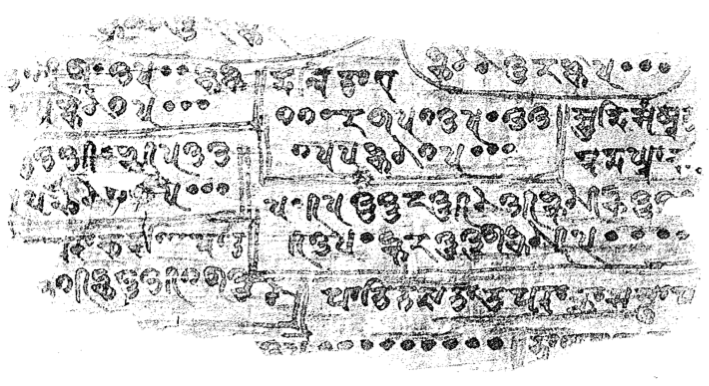
\includegraphics[scale=0.5]{bakhshali}
\end{figure}

U modernoj notaciji, algoritam kaže da za izračunati kvadratni korijen broja $q$ treba krenuti s aproksimacijom $x_0$ i zatim izračunati,
za $n\geq 0$,
\begin{align}
    a_n\: &=\: \frac{q-x^2_n}{2x_n}\\
    x_{n+1}\: &=\:x_n + a_n - \frac{a^2_n}{2(x_n + a_n)}\text.%\\
    %q\: &=\:x^2_{n+1} - \left[\frac{a^2_n}{2(x_n + a_n)}\right]^2\text.
\end{align}

Slično kao i u starobabilonskom slučaju, nema nikakvih indikacija da su staroindijski matematičari ikada iterirali gornje formule više od jedanput.
No, upravo u iteraciji leži najveća moć ove indijske metode --- algoritam kvartično konvergira\footnote{Svaka iteracija
učetverostručuje broj točnih značajnih znamenki,
pod uvjetom da nam je realna računalna aritmetika dovoljno precizna ili da radimo u racionalnoj aritmetici proizvoljne preciznosti.
Za usporedbu, poznata Newton-Raphsonova iteracijska shema konvergira kvadratno.}! Nijedan algoritam
slične efikasnosti nije bio poznat u Europi sve do 18.\ stoljeća.

% \begin{teorem}
%     Bakhshali algoritam za račun kvadratnog korijena kvartično konvergira.
% \end{teorem}
% \begin{proof}
    
% \end{proof}

\section{Moderniji pristupi}
\citat{\begin{otherlanguage}{english}
    Steve Russell certainly didn't know that his Spacewar was using a symplectic integrator.
That term wasn't invented until years later. It is serendipity that the shortest machine language program has the best numerical properties.
\end{otherlanguage}}
{Cleve Moler~\cite{spacewar}}

U ovom odjeljku ćemo razmatrati neke novije pristupe računu korijena, pri čemu mislimo uglavnom na algoritme prilagođene
izvršavanju na digitalnim računalima. Umjesto iscrpnog povijesnog pregleda svih varijanti implementiranih algoritama, usredotočit ćemo se na
nekolicinu \textsl{sui generis} algoritama i njihovih implementacija, analizirajući
njihova numerička svojstva i uspoređujući ih s onima iz odjeljka~\ref{sec:hist}.

\subsection{Algoritam s dvije varijable}
Potreba za računom kvadratnog korijena javila se vrlo rano u povijesti digitalnih računala i odgovarajuće rutine u strojnom jeziku
su ubrzo bile implementirane za računala poput EDSAC-a početkom 1950-ih godina~\cite{gower}. Takva računala tipično nisu imala ugrađen
hardver za brzu aritmetiku s pomičnim zarezom niti su podržavala instrukciju dijeljenja, pa su se tražile metode koje mogu u potpunosti
izbjeći dijeljenje i po mogućnosti koristiti samo operacije zbrajanja te bitnovnog posmaka.

Jedna takva rana metoda dolazi od ekipe predvođene Wilkesom\footnote{TODO} sa sveučilišta u Cambridgeu odgovorne za EDSAC,
inače prvo računalo s pohranjivanjem programa~\cite[str.~32]{ribaric}. Metoda je iterativna i koristi \emph{dvije} varijable te 
u potpunosti zadovoljava spomenute specifikacije. To uspijeva zahvaljujući nekim osnovnim rezultatima koje ćemo sada izvesti za
malo općenitiji slučaj izračunavanja $y/x^{1/n},\,n\in\mathbb{N}$, gdje pretpostavljamo da nas zanimaju samo pozitivni cjelobrojni rezultati, pa
je riječ o funkciji s domenom u $\mathbb{N}^2$ i kodomenom u $\mathbb N$\footnote{Ovo se može interpretirati kao račun u aritmetici
s \emph{fiksnim} zarezom, uz odgovarajuća skaliranja na početku i kraju, što je bilo uobičajeno za rana računala. Pritom želimo da algoritam
računa rezultat do na točnost $2^{-(w-1)}$, gdje je $w$ duljina riječi u bitovima, jer tako osiguravamo točan rezultat u smislu aritmetike
s fiksnim zarezom.}.

Promotrimo dvostruko iterativni proces u varijablama $a_k$ i $c_k$:
\begin{align}
        a_{k+1} &= a_k(1 + \alpha c_k)\label{eq:iter1}\\
        (y^n / x)(1 + c_{k+1}) &= a^n_{k+1}\label{eq:iter2}\text.
\end{align}
Ako $c_k\to 0$ za $k\to\infty$, onda očito vrijedi $a_k\to y/x^{1/n}$ te iz \eqref{eq:iter1} i \eqref{eq:iter2} lako izvodimo
\begin{equation}
    c_{k+1} = (1+c_k)(1+\alpha c_k)^n - 1\text.
\end{equation}
Bitno je da osiguramo konvergenciju; može se pokazati da ako $y^2<x<1$ (skalirano), za $|c_k|<1$ negativan imamo
\begin{equation}\label{eq:edsacscale}
    -1\leq c_{k+1}\leq(1+c_k)e^{-c_k}-1<0\text.
\end{equation}
Odabirom $\alpha=-1/n$ dobivamo kvadratnu konvergenciju ovog sustava~\cite{gower}.

Uvrštavanjem u \eqref{eq:iter1} i \eqref{eq:iter2}, dobivamo:
\begin{align}
    a_{k+1} &= a_k(1-c_k/n)\\
    c_{k+1} &= (1+c_k)(1-c_k/n)^n - 1\text.
\end{align}
Sada općenito vidimo da iz \eqref{eq:edsacscale} slijedi
da su sve vrijednosti niza $c_k$ negativne te da taj niz konvergira ka $0$. Iz \eqref{eq:iter2} pak dobivamo
$|a_k|^n<|y^n/x|$, iz čega možemo zaključiti da je $|a_k|<1$ (skalirano) čim je konačan rezultat isto takav.

Za dobiti formule specifično za račun kvadratnog korijena od $x$, odabiremo $a_0=y=x$ i $c_0=x-1$ te $n=2$, što nam daje:
% \begin{equation}
%     \begin{aligned}\label{eq:sqrtedsac}
%         a_{k+1} &= a_k\left(1-\frac12 c_k\right)\\
%         c_{k+1} &= \frac14 c^2_k(c_k-3)\text.
%     \end{aligned}
% \end{equation}
\begin{equation}
\left.
    \begin{array}{cc}
    \label{eq:sqrtedsac}
        a_{k+1} &= a_k\left(1-\frac12 c_k\right)\\
        c_{k+1} &= \frac14 c^2_k(c_k-3)\text.
\end{array}\right\}
\end{equation}
U ovom posebnom slučaju se konvergencija $a_k\to\sqrt x$ može lako provjeriti direktno po definiciji konvergencije
niza koji je monotono padajući (unutar legalnog raspona $x$-a vrijedi da su sve $c_k$ vrijednosti negativne te rastu tj.
apsolutna vrijednost niza pada) koristeći gornje rezultate o omeđenosti međurezultata; no, uočimo da to možemo pokazati
samo za $0\leq x<3$ po gornjem odabiru početnih uvjeta --- to je jedini raspon unutar kojeg je ova metoda primjenjiva (što se tiče korijena).

Ne samo da ova metoda ima relativno malu stvarnu domenu primjene, ona se također radi preciznosti često mora ograničiti još i više.
Vidimo da je iteriranje sustava \eqref{eq:sqrtedsac} moguće korištenjem množenja, dijeljenja s potencijama od $2$ te zbrajanja i oduzimanja, što
je lako za implementirati na svim procesorima. Ipak, ova metoda, zbog korištenja dvije iteracijske varijable, može akumulirati greške za razliku
od starobabilonske metode. Konvergencija za račun korijena ovom metodom se usporava što je $x$ manji, što znači da bi trebali pred-skalirati argument
što je više moguće (do gornje granice duljine riječi), obaviti račun i na kraju skalirati natrag; štoviše, nužno je
skalirati argument tako da vrijedi $0<x<1$ (skalirano) radi osiguravanja da će konačan rezultat biti $<1$ (skalirano), čime dobivamo
traženu garanciju strojne (u smislu fiksnog zareza) preciznosti. 
Faktor skaliranja bi trebao biti parna potencija od $2$,
kako bi račun korijena bez gubitka prepolovio eksponent.

Iz svega navedenog možemo uočiti da je područje konvergencije ovog algoritma, pogotovo za nama najzanimljiviji slučaj $n=2$, izrazito usko
(u tom slučaju vidimo da je riječ o podskupu od $\{x\mid x\in\left[0,3\right>\}$ za kojeg jedino i možemo primijeniti ovaj algoritam), pa je
zaista bitno primijeniti dosta pred- i post-procesiranja kako bi se izvuklo maksimalno preciznosti iz ovog algoritma.
Gower u \cite{gower} preporučuje ciljni raspon $(\frac12)^n\leq x<1$.
Za računala za koja je
ovaj algoritam bio
namijenjen, to je bila i jedina moguća relativno efikasna opcija.

\subsection{Algoritam bit-po-bit}
Sada ćemo proučiti jednu široko poznatu i implementiranu metodu za račun kvadratnog korijena, najčešće opet domene i kodomene u
$\mathbb{N}$, iako se često koristi s odgovarajućim skaliranjem i za "realne" brojeve
 na platformama gdje je moguća jedino aritmetika s fiksnim zarezom; mi ćemo podrazumijevati da radimo samo nad $\mathbb N$, pa ustvari
 dajemo algoritam za račun $\lfloor\sqrt x\rfloor$.

Riječ je o metodi kojom ljudi mogu dosta efikasno na papiru izračunati korijen, iako je sporija od svih prije obrađenih zbog toga
što u svakoj iteraciji daje samo jednu novu znamenku rezultata. Ipak, popularna je i dandanas upravo zbog svoje jednostavnosti te je
poznato da su neki rani ručni kalkulatori, poput Napierovih kosti (17.\ st.), koristili ovu metodu.
 Opisat ćemo je primjerom
u dekadskom brojevnom sustavu, a nakon toga formalizirati točan postupak za nama posebno zanimljiv binarni sustav.

\primjer{Izračunati $\sqrt{819}$.}
{Kako smo u dekadskom sustavu, znamo da troznamenkasti brojevi mogu imati najviše dvoznamekasti korijen; općenito, $k$-znamenkasti broj
može imati najviše $\lceil\frac{k}{2}\rceil$-znamenkasti korijen. Mi u biti želimo "riješiti jednadžbu" $(10x+y)^2+z=819$ za $x$ i $y$, gdje je 
"ostatak" $z$ potreban jer očekujemo da nam argument neće biti savršeni kvadrat. U tu svrhu krećemo od najznačajnije znamenke rješenja
$x$ --- koja je najveća znamenka koja, kvadrirana i pomnožena sa $100$, daje broj manji ili jednak $891$? Nalazimo da je to $x=2$, pa
uvrstimo to u jednadžbu i tražimo dalje $y$. Budući smo razriješili najznačajniji dio rezultata, možemo oduzeti dobiveni $400$ od $819$,
dobiti $40y+y^2+z=419$
i nastaviti pretragu kao prije. Tako nalazimo $y=8$ i, kako uvrštavanje u jednadžbu ne daje točno $419$,
znamo da imamo "ostatak" $z>0$. No, nama on nije bitan budući da ustvari računamo $\lfloor\sqrt{819}\rfloor$, pa je
 dovoljno vratiti naš dobiveni rezultat kao konačno rješenje.}

\subsubsection{Općenit pseudokod}
Općenito, ovaj algoritam se svodi na iterativno traženje najvećeg jednozamenkastog
broja koji zadovoljava da mu je izračunata vrijednost preostalog dijela multinomne jednadžbe manja ili jednaka (preostalom) argumentu, sve
dok ne odredimo vrijednosti svih nepoznanica.

Možemo pokušati formalizirati ovaj pristup za slučaj baze $2$, koja nam je jedina zanimljiva radi implementacije na računalu, na temelju
jednostavne opservacije da je korijen broja $N$ ili jednak korijenu $N-1$ ili za jedan manji od njega. Obična indukcija po $N$ nam dokazuje
ovaj rezultat, no očito je riječ o presporom načinu računanja korijena, budući bi bilo potrebno napraviti onoliko \emph{rekurzivnih}
poziva koliki je $N$, sve do dolaska do baznog slučaja za $1$, uz još dodatnu provjeru kvadriranjem na kraju koja osigurava da ne vratimo
\textsl{off-by-one} rezultat! Jasno, ovakvo nešto ne dolazi u obzir, ali sada barem imamo neku ideju na čemu temeljiti dokaz, samo nam treba
"brža" indukcija.

Tvrdimo da je moguće doći do istog rezultata koristeći, umjesto opetovanog dekrementiranja argumenta u koraku, njegovo dijeljenje s $4$
tj.\ bitovni posmak za $2$ udesno, što dovodi do vremenske složenosti $O(\lg\lg N)$ u usporedbi s prethodnom $O(\lg N)$. Osnovna ideja je
da mi na temelju izračunatog korijena od $\lfloor\frac{N}{4}\rfloor$ možemo dobiti korijen od $N$, što opravdava korištenje potpune
indukcije na $N$ u svrhu dokaza ovog korisnijeg rezultata. Za provesti tu indukciju, moramo prvo navesti neke elementarne rezultate
na koje ćemo se pozvati (u donjim iskazima pretpostavljamo da $\mathbb{N}$ uključuje $0$).

\begin{lema}
    Za sve $a,n\in\mathbb{N}$ vrijedi:
    \begin{equation}\label{lm:1}
        a=\left\lfloor\frac{a}{n}\right\rfloor\cdot n + a \bmod n\text.
    \end{equation}
\end{lema}

\begin{lema}
    Za sve $a,n\in\mathbb{N}$ vrijedi:
    \begin{equation}\label{lm:2}
        0 \leq a \bmod n \land a \bmod n < n\text.
    \end{equation}
\end{lema}

\begin{teorem}\label{tm:isqrt1}
    Korijen od $x\in\mathbb N$ je ili $2r$ ili $2r+1$, gdje $r^2\leq\left\lfloor\frac{x}{4}\right\rfloor < (r+1)^2$. Preciznije,
    ako je $x < (2r+1)^2$, tada je korijen $2r$, a inače je korijen $2r+1$~\cite{sqrtproof}.
\end{teorem}
\begin{proof}
    Potpunom indukcijom po $x$. U baznom slučaju, za $x=0$, imamo da je korijen dakako $0$.

    Pretpostavka indukcije nam je da kada tvrdnja vrijedi za sve brojeve manje od $x$, tada ona vrijedi i za $x$.
    Obzirom da imamo dva različita slučaja u tvrdnji, korak provodimo po slučajevima.
    \paragraph{Slučaj 1: $x<(2r+1)^2$}
    
    U ovom slučaju tvrdimo da je korijen $2r$, pa valja pokazati da vrijedi $(2r)^2\leq x < (2r+1)^2$. Desnu nejednakost već pretpostavljamo,
    a prva slijedi osnovnim algebarskim manipulacijama:
    \begin{align*}
        r^2 &\leq \left\lfloor\frac{x}{4}\right\rfloor &\\
        r^2\cdot 4 &\leq \left\lfloor\frac{x}{4}\cdot 4\right\rfloor &\\
        (2r)^2 &\leq \left\lfloor\frac{x}{4}\right\rfloor\cdot 4 &\\
        (2r)^2 &\leq (x - x \bmod 4) & \text{po \eqref{lm:1}}\\
        x - x \bmod 4 &\leq x & \text{po \eqref{lm:2}}\\
        (2r)^2 &\leq  x\text.&
    \end{align*} %TODO: ovdje možda staviti brace desno na iz predzadnje dvije činjenice, koristeći NiceArray https://tex.stackexchange.com/q/621786

    \paragraph{Slučaj 2: $x \geq (2r+1)^2$}

    Sada tvrdimo da je korijem $2r+1$, pa dokazujemo da vrijedi $(2r+1)^2 \leq x < (2r+2)^2$. Prva nejednakost je sada trivijalno zadovoljena,
    a za drugu možemo postupiti ovako:
    \begin{align*}
        \left\lfloor\frac{x}{4}\right\rfloor &< (r+1)^2 & \text{po pretpostavci indukcije}\\
        \left\lfloor\frac{x}{4}\right\rfloor + 1 &\leq (r+1)^2 \bigg/\cdot 4 &\\
        \left\lfloor\frac{x}{4}\right\rfloor\cdot 4 + 4 &\leq (r+1)^2\cdot 4 = (2r+2)^2 &\\
        x - x \bmod 4 + 4 &\leq (2r+2)^2 & \text{po \eqref{lm:1}}\\
        x &\leq (2r+2)^2 + x \bmod 4 - 4 &\\
        (2r+2)^2 + x \bmod 4 - 4 &< (2r+2)^2 & \text{po \eqref{lm:2}}\\
        x &< (2r+2)^2\text.&
    \end{align*}
\end{proof}

Sada imamo zgodan algoritam za računati korijene koji je direktno primjenjiv i za ručno računanje, iako najvjerojatnije zahtijeva papir
za pamćenje rezultata za veće argumente. Vidimo da algoritam napreduje dijeljenjem preostalog dijela argumenta (u potproblemu) s $4$, što
odgovara bitovnom posmaku za 2 udesno i stoga se lako vizualizira i izvodi u računalu, iako za ljude možda nije najprirordnije raditi u bazi $2$.
U tom slučaju računamo u bazi $10$ i, umjesto $4$, za djelitelja odabiremo $100$ kao prvi savršeni kvadrat te baze i svi ostali rezultati slijede
na analogan način. Pseudokod generičkog algoritma za bazu $B$ glasi:
\begin{algorithm}
    \floatname{algorithm}{Algoritam}
    \caption{Algoritam $\mathsf{isqrt}$ za cjelobrojni kvadratni korijen od $N$ u bazi $B$}\label{alg:isqrt1}
    \begin{algorithmic}
    \Require $N \geq 0$
    \If{$N = 0$}
        \State $rezultat \gets 0$
    \Else
        \State $z \gets \left\lfloor\dfrac{N}{B^2}\right\rfloor$
        \State $r_2 \gets B \cdot \mathsf{isqrt}(z)$
        \State $r_3 \gets r_2 + 1$
        \If{$N < r_3^2$}
            \State $rezultat \gets r_2$
        \Else
            \State $rezultat \gets r_3$
        \EndIf
    \EndIf
    \end{algorithmic}
\end{algorithm}

Jasno, ovo je čisto rekurzivna implementacija teorema \eqref{tm:isqrt1} dokazanog indukcijom za koju ne očekujemo jako dobre performanse upravo zbog
uporabe rekurzije. Usredotočimo se na slučaj za $B=2$ i prevedimo algoritam \ref{alg:isqrt1} u iterativni pseudokod uz nekoliko optimizacija:
\begin{algorithm}
    \floatname{algorithm}{Algoritam}
    \caption{Algoritam $\mathsf{isqrt}$ za $B=2$, iterativna varijanta za $32$-bitnu arhitekturu~\cite{guysqrt}}\label{alg:isqrt2}
    \begin{algorithmic}[1]
    \Require $N \geq 0$
    \State $op \gets N$
    \State $rezultat \gets 0$
    \State $jedinica \gets 2^{30}$
    \While{$jedinica > op$}
        \State $jedinica \gets \left\lfloor\frac{jedinica}{4}\right\rfloor$
    \EndWhile

    \While{$jedinica\neq 0$}
        \If{$op \geq rezultat + jedinica$}
            \State $op \gets op - (rezultat + jedinica)$
            \State $rezultat \gets rezultat + 2 \cdot jedinica$\label{line:rezupd}
        \EndIf
        \State $rezultat \gets \left\lfloor\frac{rezultat}{2}\right\rfloor$
        \State $jedinica \gets \left\lfloor\frac{jedinica}{4}\right\rfloor$
    \EndWhile
    \end{algorithmic}
\end{algorithm}

Objasnimo pobliže što se dogodilo u transformaciji iz algoritma \ref{alg:isqrt1} u algoritam \ref{alg:isqrt2}. Prva očita stvar je da, umjesto kretanja
od točno najvišeg ne-nula bita od $N$\footnote{U praksi se ovaj algoritam izvodi na računalima gdje ćemo, zbog fiksnih
i relativno malih širina registara, uvijek kretati od najviše bitovne pozicije (ovo ima smisla do oko $32$ bita).
Naravno da onda postoje i varijante u kojima se pokušava na razne načine
zaobići potreba prolaska od najvišeg bita uz obavljanje cijelog računa svaki put, što može dovesti do ubrzanja, ali samo uz povećanje
prostorne složenosti jer nam tada treba barem nekakva konstantna tablica vrijednosti u memoriji.
Jedan takav algoritam, zasnovan na tablici i malom broju računskih operacija,
bit će obrađen zadnji.}, što bi zahtijevalo i inicijalno izračunavanje indeksa te pozicije, mi jednostavno možemo krenuti od najvišeg bita registra.
Preciznije, budući da znamo da ćemo u koraku dijeliti s $4$ tj.\ posmaknuti sve bitove za $2$ mjesta udesno (u niskorazinskim implementacijama), dovoljno
je započeti na najznačajnijoj grupi od dva bita, s tim da mi pamtimo \emph{niži} indeks i postavljamo jedinicu tamo.  To nam omogućuje laganu provjeru
kraja algoritma: kada je ostatak bitova iz $jedinica$ kompletno u $0$, više nema potrebe ništa računati i prekidamo algoritam.

Dualno, ne zanimaju nas ni najviši $0$-bitovi iz $N$ jer oni ne mogu doprinijeti korijenu, pa se pomičemo po dva bita udesno dok ne "udarimo" u neki 
par ne-nula bitova iz $N$. U tom trenutku dakle, nakon završetka prve \textsl{while} petlje,
znamo par indeksa među kojima je indeks pozicije najvišeg bita u $N$. Sada idemo, unutar iduće petlje, obaviti sve korake dok ne iscrpimo
sve relevantne parove bitova. Ovdje je ključna optimizacija držanje trenutne (reducirane) verzije argumenta $N$ u varijabli $op$ jer nam omogućuje
da, u slučaju da vrijedi $N \ge (2r+1)^2$ u algoritmu \ref{alg:isqrt1} na nekoj razini poziva, lako korigiramo rezultat. Trik je u tome da sada
\emph{uopće ne kvadriramo} unutar te provjere, jer uočavamo da je proširen izraz $(2r+1)^2=4r^2+4r+1$ uvijek s postavljenim najnižim bitom, a kako
mi napredujemo kroz korake upravo dijeljenjem $jedinice$ s $4$ (preostali faktori u izrazu su umnošci od $4$), znamo da smo
do ovog koraka petlje u $rezultat$ već smjestili sve niže bitove rješenja. Zato test $op\geq rezultat+jedinica$ ispravno testira je li se dogodio
odgovarajući preljev. Preostaje još "popraviti" varijable: $op$ se mora umanjiti za $rezultat+jedinica$ jer je 
"bit viška" već doprinio rezultatu; ukoliko viška nema, $op$ se ne mijenja jer nije mogao biti postavljen ni jedan novi bit rezultata.
Važno je da se u liniji \ref{line:rezupd} $rezultat$ uveća za $2\cdot jedinica$, jer mi pamtimo jedinicu na nižoj poziciji para, a trebamo
postaviti bit na višoj poziciji. Na samom kraju petlje jednostavno posmičemo bitove u odgovarajućim varijablama, gdje je bitno da se $rezultat$
pomiče samo za jedno mjesto udesno jer mi u svakom koraku dobivamo točno jedan novi bit rezultata ($0$ ako nema preljeva), iz čega proizlazi ime
ove sekcije odnosno algoritma.

Iako se čini da ovaj algoritam ne napreduje suviše brzo, njegova je glavna prednost to što ima fiksan broj iteracija petlje
(ovisan samo o duljini registara ciljne arhitekture) i stoga relativno lako odredivo ukupno
vrijeme izvršavanja na jednostavnijim, danas uglavnom ugradbenim arhitekturama.

\subsection{CPython-ov algoritam}
\citat{The integer square root is a common number-theoretic primitive, useful for example in primality testing.
This is something I've had to code up myself multiple times, and is also something that's quite easy to get wrong,
or implement in a way that's inefficient for large inputs~\cite{mdickisqrt}.}{Mark Dickinson}

Trenutna verzija CPythona --- referentne implementacije virtualnog stroja za programski jezik Python --- koristi zanimljivu varijantu 
algoritma \ref{alg:isqrt2} za račun cjelobrojnog kvadratnog korijena~\cite{Cpythonisqrt}. Naime, radi se o \emph{adaptivnom} algoritmu
koji umjesto posmaka za fiksni broj mjesta koristi varijabilni posmak $s$ koji se smanjuje kako algoritam napreduje. Iteracije se baziraju
na Newtonovoj metodi i koristi se puno brža metoda u posebnom slučaju kada je argument manji od $2^{64}$; naime, Python interno podržava
cjelobrojnu aritmetiku proizvoljne preciznosti, no raditi račun u proizvoljno visokoj preciznosti kada bi se mogao izvesti i u puno manjoj
(idealno nativno hardverskoj) je rastrošno, pa algoritam ustvari adaptivno povećava preciznost računa. Također postoji posebna, vrlo kratka
i efikasna varijanta koja se sastoji samo od najosnovnijih aritmetičkih operacija i ne sadrži grananja.
U samom Pythonu, ova funkcija je dostupna kao \texttt{math.isqrt} od
verzije 3.8.

TODO: kratka skica dokaza iz komentara cpythona?





\subsection{Korijen iz recipročnog korijena}
\section{Implementacije i usporedbe}
%TODO: ubaci primjere i za sve ostale, povijesne sqrt metode! Ima dosta toga u Knuth članku, Fowler...

\printbibliography

\end{document}